%%%%%%%%%%%%%%%%%%%%%%%%%%%%%%%%%%%%%%%%%%%%%%%%%%%%%%%%%%%%%%%%%%%%%%%%%%%%%%%%%%%%%
\documentclass[11pt,a4paper,ssfamily]{exam}                                        %%
\usepackage[numbers,sort&compress]{natbib}                                         %%
\usepackage[utf8]{inputenc}                                                        %%
\renewcommand{\baselinestretch}{1.15}                                              %%
\usepackage{epsfig}                                                                %%
\usepackage{graphicx}                                                              %%
\usepackage{makeidx}                                                               %%
\usepackage{hyperref}                                                              %%
\usepackage{multicol}                                                              %%
\usepackage{multirow}                                                              %%
\newcommand{\listfont}{\bf\fontencoding{OT1}\sffamily\large}                       %%
\newcommand{\titlesfont}{\fontencoding{OT1}\sffamily\large}                        %%
\renewcommand{\baselinestretch}{1.24}                                              %%
\usepackage{tabularx}                                                              %%
\usepackage[table]{xcolor}% http://ctan.org/pkg/xcolor                             %%
\newcolumntype{C}{>{\centering\arraybackslash}X}                                   %%
\usepackage{pdfpages}                                                              %%
                                                                                   %%
\begin{document}                                                                   %%
                                                                                   %%
\sffamily                                                                          %%
\pagestyle{empty}                                                                  %%
                                                                                   %%
\begin{center}                                                                     %%
\begin{tabularx}{\textwidth}{cCc}                                                  %%
\multirow{3}{21mm}{
\includegraphics[height=2.18cm]{./logo_unicamp.pdf}}            %%
        &  UNIVERSIDADE ESTADUAL DE CAMPINAS   &                                   %%
\multirow{3}{21mm}{
\includegraphics[height=2.18cm]{./logo_iq.pdf}} \\              %%
        &         INSTITUTO DE QUÍMICA         &     \\                            %%
       & \textbf{PLANO DE DESENVOLVIMENTO DE DISCIPLINA} \\                        %%
\end{tabularx}                                                                     %%
\vspace{0.5cm}                                                                     %%
\end{center}                                                                       %%
\begin{center}                                                                     %%
\textbf{                                                                           %%
%%%%%%%%%%%%%%%%%%%%%%%% Período %%%%%%%%%%%%%%%%%%%%%%%%%%%%%%%%%%%%%%%%%%%%%%%%%%%%
1$^\textrm{\underline{o}}$ Semestre - 2019
%%%%%%%%%%%%%%%%%%%%%%%%%%%%%%%%%%%%%%%%%%%%%%%%%%%%%%%%%%%%%%%%%%%%%%%%%%%%%%%%%%%%%
}\\                                                                                %%
\vspace{0.5cm}                                                                     %%
\begin{tabularx}{\textwidth}{|l|X|}                                                %%
\hline                                                                             %%
\multicolumn{2}{|c|}{\cellcolor{lightgray} \textbf{\Large{Disciplina}}} \\         %%
\hline                                                                             %%
\cellcolor{lightgray}\textbf{Código}    & \cellcolor{lightgray}\textbf{Nome} \\    %%
\hline                                                                             %%
%%%%%%%%%%%%%%%%%%%%% Título da disciplina %%%%%%%%%%%%%%%%%%%%%%%%%%%%%%%%%%%%%%%%%%
QF637     &  Introdução à Espectroscopia e à Termodinâmica Estatística \\
%%%%%%%%%%%%%%%%%%%%%%%%%%%%%%%%%%%%%%%%%%%%%%%%%%%%%%%%%%%%%%%%%%%%%%%%%%%%%%%%%%%%%
\hline                                                                             %%
\end{tabularx}\\                                                                   %%
\vspace{0.5cm}                                                                     %%
\begin{tabularx}{\textwidth}{|l|l|X|}                                              %%
\hline                                                                             %%
\cellcolor{lightgray}\textbf{Turmas} &\cellcolor{lightgray}                        %%
\textbf{Horário} &\cellcolor{lightgray}\textbf{Local} \\                           %%
\hline                                                                             %%
%%%%%%%%%%%%%%%%%% Turmas, horários e locais %%%%%%%%%%%%%%%%%%%%%%%%%%%%%%%%%%%%%%%%
A    &  Seg: 16-18; Qua: 8-10 & IQ03 \\\hline
%%%%%%%%%%%%%%%%%%%%%%%%%%%%%%%%%%%%%%%%%%%%%%%%%%%%%%%%%%%%%%%%%%%%%%%%%%%%%%%%%%%%%
\end{tabularx}                                                                     %%
Disponível em                                                                      %%
\href{https://www.iqm.unicamp.br/gradua\%C3\%A7\%C3\%A3o}                          %%
{https://www.iqm.unicamp.br/gradua\%C3\%A7\%C3\%A3o}\\                             %%
\vspace{0.5cm}                                                                     %%
\begin{tabularx}{\textwidth}{|X|}                                                  %%
\hline                                                                             %%
\cellcolor{lightgray}\textbf{Docentes} \\                                          %%
\hline                                                                             %%
%%%%%%%%%%%%%%%%% Docentes %%%%%%%%%%%%%%%%%%%%%%%%%%%%%%%%%%%%%%%%%%%%%%%%%%%%%%%%%%
Leandro Martínez - leandro@iqm.unicamp.br - Sala H312 \\\hline
%%%%%%%%%%%%%%%%%%%%%%%%%%%%%%%%%%%%%%%%%%%%%%%%%%%%%%%%%%%%%%%%%%%%%%%%%%%%%%%%%%%%%
\end{tabularx}\\                                                                   %%
\vspace{0.5cm}                                                                     %%
\begin{tabularx}{\textwidth}{|X|}                                                  %%
\hline                                                                             %%
\cellcolor{lightgray}\textbf{Critérios de Avaliação e Aprovação} \\                %%
\hline                                                                             %%
\begin{minipage}[t]{0.95\columnwidth}\small{                                       %%
%%%%%%%%%%%%%%%%% Critérios de avaliação %%%%%%%%%%%%%%%%%%%%%%%%%%%%%%%%%%%%%%%%%%%%
A disciplina contará com duas provas, cada uma correspondente a um dos
tópicos: Espectroscopia ou Termodinâmica Estatística. Para ser aprovado
sem a realização do EXAME, o aluno deve ter nota maior ou igual a 3,0 em
ambas as provas, e média aritmética de provas maior ou igual a 5,0.\\

Em caso de aprovação direta, a média de avaliações do aluno será a média
aritmética das provas.\\

Caso o aluno tenha que fazer exame em função das notas das provas, a
média de avaliações será a média aritmética da nota do exame com a média
aritmética das notas das provas.\\

O Exame abarcará todo o conteúdo da disciplina, mesmo que o aluno tenha
obtido nota maior que 5,0 em um dos tópicos.\\

Por fim, a disciplina conta com uma lista de exercícios para cada
tópico. As listas devem ser feitas a mão e entregues, e receberão uma
nota de 0 a 10, em função da quantidade de exercícios feitos. Para cada
2 exercícios que não foram feitos com cuidado, a nota cai 1 ponto.\\

A nota final da disciplina será calculada pela média geométrica da nota
da lista com a média de avaliações. Se a nota final for maior ou igual a
5,0, o aluno será aprovado. Se for menor que 5,0, o aluno será
reprovado.\\

As provas serão entregues corrigidas, e sua resolução será discutida nos
dias reservados no cronograma, exclusivamente.\\

Notas, exercícios e informações adicionais: 
\href{http://leandro.iqm.unicamp.br}{http://leandro.iqm.unicamp.br}, 
no link ``Material Didático''.
%%%%%%%%%%%%%%%%%%%%%%%%%%%%%%%%%%%%%%%%%%%%%%%%%%%%%%%%%%%%%%%%%%%%%%%%%%%%%%%%%%%%%
}\end{minipage}\vspace{0.1cm}\\                                                    %%
\hline                                                                             %%
\end{tabularx}\\                                                                   %%
\vspace{0.5cm}                                                                     %%
\begin{tabularx}{\textwidth}{|X|}                                                  %%
\hline                                                                             %%
\cellcolor{lightgray}\textbf{Calendário} \\                                        %%
\hline                                                                             %%
\begin{minipage}[t]{0.95\columnwidth}\vspace{0.1cm}\small{                         %%
%%%%%%%%%%%%%%%%%%%%%% Cronograma %%%%%%%%%%%%%%%%%%%%%%%%%%%%%%%%%%%%%%%%%%%%%%%%%%%
\begin{center}\begin{tabular}{ccc}
\hline
\multicolumn{3}{c}{{\bf Cronograma}} \\
\hline
Mês   &   Dia                &      Atividade          \\
\hline
Fevereiro  &
   27      &  Apresentação/Aula      \\
\hline
\multirow{2}{15mm}{\rotatebox{0}{\mbox{Março}}}  &
   4,6     &  Feriado                \\
 & 11,13,18,20,25,27  &  Aulas       \\
\hline
\multirow{1}{15mm}{\rotatebox{0}{\mbox{Abril}}}  &
   1,3,8,10,15,17,22,24,29  &  Aulas                  \\
\hline
\multirow{6}{15mm}{\rotatebox{0}{\mbox{Maio}}}  &
   1       &  Feriado  \\
 & 6       &  Prova 1 \\
 & 8       &  Correção da Prova 1 / Aula \\
 & 13,15,20 & Aulas \\
 & 22      & Não haverá aula.\\
 & 27,29   &  Aulas  \\ 
\hline
\multirow{3}{15mm}{\rotatebox{0}{\mbox{Junho}}}  &
   3,5,10,12,17,19,24,26   &  Aulas   \\
 & 24      &  Prova 2   \\
 & 26      &  Correção da Prova 2 \\ 
\hline
\multirow{2}{15mm}{\rotatebox{0}{\mbox{Julho}}}  &
   1 - 6      &  Semana de Estudos   \\
 & 8      &  Exame  \\
\hline
\end{tabular}\end{center}
%%%%%%%%%%%%%%%%%%%%%%%%%%%%%%%%%%%%%%%%%%%%%%%%%%%%%%%%%%%%%%%%%%%%%%%%%%%%%%%%%%%%%
}\end{minipage}\vspace{0.1cm}\\                                                    %%
\hline                                                                             %%
\end{tabularx}\\                                                                   %%
\vspace{0.5cm}                                                                     %%
\begin{tabularx}{\textwidth}{|X|}                                                  %%
\hline                                                                             %%
\cellcolor{lightgray}\textbf{Outras informações relevantes} \\                     %%
\hline                                                                             %%
\begin{minipage}[t]{0.95\columnwidth}\vspace{0.1cm}\small{                         %%
%%%%%%%%%%%%%%%%%% Outras informações relevantes %%%%%%%%%%%%%%%%%%%%%%%%%%%%%%%%%%%%

%%%%%%%%%%%%%%%%%%%%%%%%%%%%%%%%%%%%%%%%%%%%%%%%%%%%%%%%%%%%%%%%%%%%%%%%%%%%%%%%%%%%%
}\end{minipage}\vspace{0.1cm}\\                                                    %%
\hline                                                                             %%
\end{tabularx}\\                                                                   %%
\vspace{0.5cm}                                                                     %%
SEGUEM A EMENTA, PROGRAMA E BIBLIOGRAFIA                                           %%
%%%%%%%%%%%%%%%%%%%% PDF da ementa e programa %%%%%%%%%%%%%%%%%%%%%%%%%%%%%%%%%%%%%%%
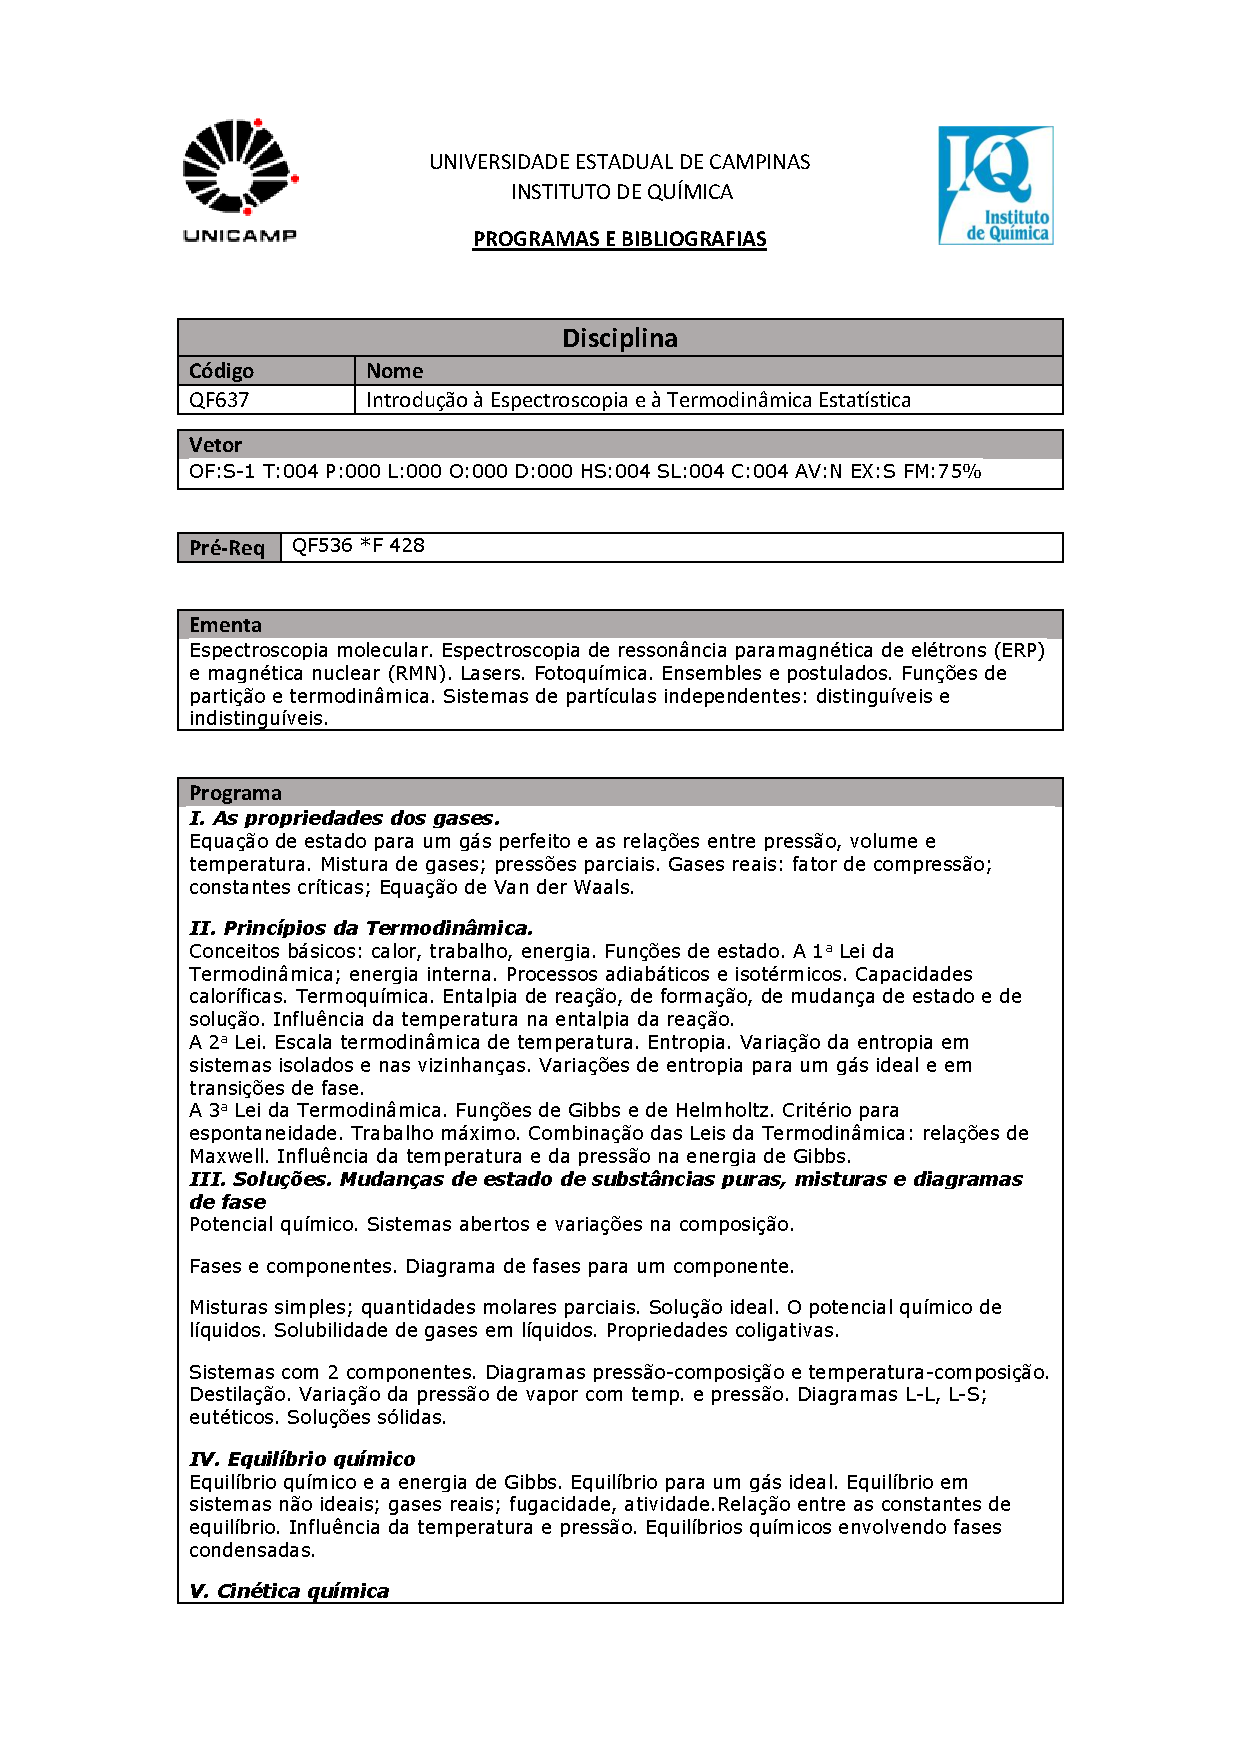
\includepdf[pages={1-},scale=1]{./QF637_programa.pdf}
%%%%%%%%%%%%%%%%%%%%%%%%%%%%%%%%%%%%%%%%%%%%%%%%%%%%%%%%%%%%%%%%%%%%%%%%%%%%%%%%%%%%%
\end{center}
\end{document}



